% =========================================================
\chapter{Lecture 4 : Mandatory Access Control}
% =========================================================

\begin{rembox}[title=In a nutshell]
\textbf{What is this lecture about?} In \textbf{MAC}, it is not the owner but a
\textbf{central policy} that decides, and nobody can override it. We study three classic
``recipes'' (security models): \textbf{Bell-La Padula} to keep secrets from leaking down
(army: no read up, no write down), \textbf{BIBA} to keep bad data from corrupting good
data (bank: no read down, no write up), and the \textbf{Chinese Wall} to avoid conflicts
of interest (a consultant cannot work for Pepsi and Coca-Cola). \\
\textbf{Why is it useful?} When an organization must guarantee a property no matter what
users do (military secrets, bank records, hospitals), these models give a ready-made,
proven design. They also explain deep real-world problems: hidden leaks (\emph{covert
channels}), why declassifying documents is hard, and why unchecked user input
(\emph{sanitization}) causes SQL injections and buffer overflows.
\end{rembox}

\begin{defnbox}[title=Mandatory Access Control (MAC)]
Access to and operations on resources \textbf{are determined by the security policy}
(a central security policy assigns permissions):
\begin{itemize}
  \item the ``owner'' may not exist, or may not have the power to set permissions
        against the policy;
  \item the security policy \textbf{must} be enforced despite subjects trying to
        subvert it.
\end{itemize}
\end{defnbox}

\begin{defnbox}[title=Security model]
A \textbf{design pattern} for a specific security property or set of properties. When
faced with a standard security problem $\to$ use a well-known model!
\end{defnbox}

\begin{warnbox}[title=The devil is in the details]
Many aspects are \textbf{not covered by the model}: who are the subjects? what are the
objects? what mechanisms to use to implement it?
\end{warnbox}

\section{Bell-La Padula (BLP): protecting confidentiality}

\begin{defnbox}[title=Bell-La Padula model (BLP)]
Subjects $S$ and objects $O$ are associated to a \textbf{level} of confidentiality.
Subjects' access rights are defined (in an access control matrix) by four attributes:
\begin{itemize}
  \item \textbf{Execute} --- the subject cannot see or modify the object, but can run it;
  \item \textbf{Read} --- the subject can only see the object but cannot modify it;
  \item \textbf{Append} --- the subject cannot read the object, but can attach new
        content;
  \item \textbf{Write} --- the subject can see the object and add content or modify
        existing content.
\end{itemize}
\end{defnbox}

\begin{rembox}[title=Observe vs.\ alter]
\textbf{Observe} rights: read ($r$), write ($w$). \textbf{Alter} rights: append ($a$),
write ($w$). Write is both observe and alter.
\end{rembox}

\subsection{Security levels and dominance}

\begin{defnbox}[title=Security level (classification of objects)]
Objects are associated to a \textbf{security level}: they have a \textbf{label} and
belong to one or more \textbf{categories}.
\[
  \text{Security level} = (\text{Classification}, \{\text{set of categories}\})
\]
\begin{itemize}
  \item \textbf{Classification} --- \textbf{total order} of labels (e.g.\
        Unclassified $<$ Confidential $<$ Secret $<$ Top Secret).
  \item \textbf{Categories} --- compartments of objects with a common topic (e.g.\
        Nuclear, NATO, Crypto).
\end{itemize}
\end{defnbox}

\begin{defnbox}[title=Dominance relationship]
A security level $(l_1, c_1)$ \textbf{dominates} $(l_2, c_2)$ \textbf{if and only if}
\[
  l_1 \geq l_2 \quad\text{and}\quad c_2 \subseteq c_1 .
\]
\end{defnbox}

\begin{exbox}[title={Exercise --- Dominance}]
Labels: Admin $<$ Nurse $<$ Surgeon $<$ Doctor; categories: DEMOGRAPHICS, ANALYSIS,
RESULTS. Which statements are true?
\begin{itemize}
  \item $(D, \{\})$ dominates $(S, \{\})$
  \item $(S, \{\})$ dominates $(N, \{\text{RESULTS}\})$
  \item $(S, \{\text{DEMOGRAPHICS}, \text{RESULTS}\})$ dominates
        $(N, \{\text{DEMOGRAPHICS}\})$
  \item $(D, \{\text{ANALYSIS}, \text{RESULTS}\})$ dominates
        $(S, \{\text{DEMOGRAPHICS}\})$
\end{itemize}
What level dominates them all? What level dominates only itself?
\end{exbox}

\begin{propbox}[title=Dominance lattice]
Three key properties:
\begin{enumerate}[label=(\alph*)]
  \item dominates is \textbf{transitive};
  \item there are \textbf{top and bottom} elements;
  \item it is only a \textbf{partial} order: two levels may be incomparable (e.g.\
        $(S, \{\text{Crypto}\})$ and $(S, \{\text{Nuclear}\})$).
\end{enumerate}
\begin{center}
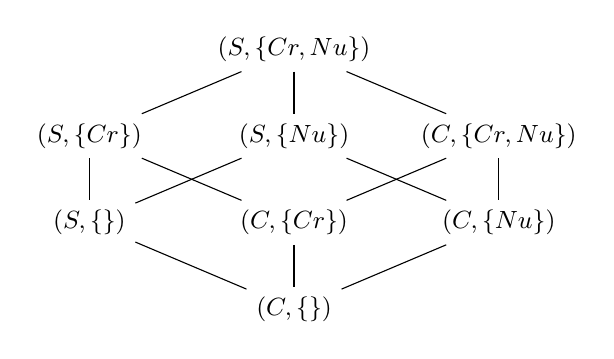
\begin{tikzpicture}[x=2.6cm, y=1.1cm, every node/.style={font=\small}]
  \node (top) at (0,3)    {$(S, \{Cr, Nu\})$};
  \node (sc)  at (-1,2)   {$(S, \{Cr\})$};
  \node (sn)  at (0,2)    {$(S, \{Nu\})$};
  \node (ccn) at (1,2)    {$(C, \{Cr, Nu\})$};
  \node (s0)  at (-1,1)   {$(S, \{\})$};
  \node (cc)  at (0,1)    {$(C, \{Cr\})$};
  \node (cn)  at (1,1)    {$(C, \{Nu\})$};
  \node (bot) at (0,0)    {$(C, \{\})$};
  \draw (top) -- (sc); \draw (top) -- (sn); \draw (top) -- (ccn);
  \draw (sc) -- (s0);  \draw (sn) -- (s0);
  \draw (sc) -- (cc);  \draw (sn) -- (cn);
  \draw (ccn) -- (cc); \draw (ccn) -- (cn);
  \draw (s0) -- (bot); \draw (cc) -- (bot); \draw (cn) -- (bot);
\end{tikzpicture} \\
{\small Labels $C < S$, categories Crypto, Nuclear: a higher node dominates every node
reachable downwards.}
\end{center}
\end{propbox}

\begin{defnbox}[title=Clearance of subjects]
\begin{itemize}
  \item \textbf{Clearance} --- maximum security level a subject has been assigned:
        $\text{level}(S_i)$ (BLP also calls this ``classification'').
  \item \textbf{Current security level} --- subjects can operate at lower security
        levels: $\text{current-level}(S_i)$.
\end{itemize}
$\text{level}(S_i)$ \textbf{must dominate} $\text{current-level}(S_i)$!
\end{defnbox}

\subsection{The three BLP properties}

\begin{defnbox}[title=Simple security property (ss-property) --- No Read Up]
If (subject, object, $r$) is a current access, then $\text{level}(\text{subject})$
\textbf{dominates} $\text{level}(\text{object})$. \\
$\Rightarrow$ \textbf{No Read Up (NRU)}: a subject cleared Secret can read Secret,
Classified, Unclassified, but not Top Secret.
\end{defnbox}

\begin{warnbox}[title=Why is the ss-property not sufficient?]
A Secret subject runs \textbf{malicious code} (Trojan) that reads Secret data (allowed
by NRU) and \textbf{writes it into an Unclassified object}, which an Unclassified subject
then reads (also allowed by NRU). Information flowed \textbf{down} without any read-up.
\end{warnbox}

\begin{defnbox}[title=Star property (*-property) --- No Write Down]
If a subject has simultaneous ``\textbf{observe}'' ($r$, $w$) access to $O_1$ and
``\textbf{alter}'' ($a$, $w$) access to $O_2$, then $\text{level}(O_2)$
\textbf{dominates} $\text{level}(O_1)$. \\
$\Rightarrow$ \textbf{No Write Down (NWD)}: a Secret subject can append to Top Secret,
read Secret and below, but cannot append/write to lower levels.
\end{defnbox}

\begin{defnbox}[title=Discretionary property (ds-property)]
If an access (subject, object, action) takes place, it \textbf{must be in the access
control matrix}. \\
Information should only be accessed on a \textbf{``need-to-know''} basis: MAC needs
\textbf{DAC} (least privilege inside the security level). Also important to protect
integrity.
\end{defnbox}

\begin{exbox}[title=BLP in the army]
\begin{itemize}
  \item An Unclassified soldier reports ``We've seen tanks moving!'' to a Secret
        officer: \textbf{allowed} (write up).
  \item The Secret officer reads a Secret document: \textbf{allowed} (read at clearance
        level).
  \item The Secret officer orders ``Attack!'' to the Unclassified soldier: \textbf{not
        allowed} (write down, against the *-property).
\end{itemize}
\end{exbox}

\begin{thmbox}[title=Basic Security Theorem]
If all state transitions are \textbf{security preserving}, and the \textbf{initial state
is secure}, then every subsequent state is secure \textbf{regardless of the inputs}. \\
If, for any individual access, (1) the ss-property, (2) the *-property and (3) the
ds-property are preserved, then security holds for any sequential composition: a
system can be analyzed in terms of \textbf{single-step transitions} of states (not
surprising: it is an induction).
\end{thmbox}

\subsection{Covert channels}

\begin{exbox}[title={What are the transitions, and what does ``read'' mean?}]
$\text{level}(s_1) = TS$, $\text{level}(s_2) = C$.
\begin{enumerate}
  \item $s_2$ creates $o_2$, so $\text{level}(o_2) = C$;
  \item $s_1$ reads $C$ and either raises the object level to $TS$ or leaves it at $C$;
  \item $s_2$ attempts to access $o_2$: \textbf{success or failure leaks 1 bit of
        information} from $TS$ to $C$!
\end{enumerate}
\end{exbox}

\begin{defnbox}[title=Covert channel]
Any channel that allows \textbf{information flows contrary to the security policy}.
\begin{itemize}
  \item \textbf{Storage channels} --- e.g.\ shared counters, ID fields, file
        metadata, etc.
  \item \textbf{Timing channels} --- e.g.\ use of CPU, load to memory (cache), queuing
        time, etc.
\end{itemize}
\end{defnbox}

\begin{propbox}[title=Covert channels and least common mechanism]
\textbf{The more resources are shared, the harder it is to eliminate covert channels}
(principle 7, least common mechanism). \\
\textbf{Mitigation}: isolation (communication with low level not possible) or adding
noise to the communication.
\begin{itemize}
  \item Hard to achieve less than 1 bit/sec.
  \item OK for documents, \textbf{NOT} OK for cryptographic keys (DoD policy:
        cryptographic keys must always be stored on dedicated hardware).
\end{itemize}
\end{propbox}

\subsection{Declassification}

\begin{defnbox}[title=Declassification]
\textbf{Remove the classification label} of an object. It is very typical and necessary
(e.g.\ the officer must eventually be able to tell the soldier ``Attack!''), and happens
\textbf{under the control of the security policy}.
\end{defnbox}

\begin{warnbox}[title=Declassification cannot be made inherently safe]
It is a \textbf{manual process} (rules about archives, historical records) and it is hard
to rule out covert channels: how to know the object does not contain secrets? In
practice: Word revision history retains deleted text; PDF ``redaction'' by overlaying
black rectangles leaves the text in the file. \textbf{Strategic adversary!}
\end{warnbox}

\begin{warnbox}[title=BLP limitations]
\begin{itemize}
  \item \textbf{Confidentiality-oriented}: does not consider integrity or availability.
  \item \textbf{State-based + single transition} model: too low-level, not expressive.
  \item The 3 security properties are \textbf{not sufficient} to ensure
        confidentiality: changes in clearance and classification can create covert
        channels, and a static system without changes is impractical.
\end{itemize}
\end{warnbox}

\section{BIBA: protecting integrity}

\begin{rembox}[title=Why integrity?]
BLP focuses on confidentiality (military / government). For \textbf{commercial services}
(banking, inventory, stock exchange, land registry, grades database, contracts,
payments), preventing fraud is about \textbf{protecting integrity}: the adversary has not
influenced the result; confidentiality is either secondary or unnecessary. \\
\textbf{Integrity is key for computer security in general}: the TCB has to have high
integrity; public key cryptography requires high integrity for confidentiality.
\end{rembox}

\begin{defnbox}[title=BIBA model]
Subjects and objects have an \textbf{integrity level} (from lowest to high integrity).
Two operations: \textbf{read} (observe) and \textbf{write} (modify). Two key (strict)
rules:
\begin{itemize}
  \item \textbf{Simple integrity (no read-down)} --- protects higher integrity
        principals from being corrupted by lower integrity level data.
  \item \textbf{*-integrity (no write-up)} --- prevents lower integrity principals from
        corrupting high integrity data.
\end{itemize}
\end{defnbox}

\begin{rembox}[title=BIBA is the dual of BLP]
BLP: no read \emph{up}, no write \emph{down} (secrets must not flow down). \\
BIBA: no read \emph{down}, no write \emph{up} (dirty data must not flow up).
\end{rembox}

\begin{exbox}[title=BIBA illustrated]
\textbf{Bank}: the director can establish a rule and every employee reads it; employees
cannot rewrite rules. \textbf{Computer}: a web application open in the browser should not
write to the file system (at most \texttt{/tmp}).
\end{exbox}

\subsection{BIBA variants}

\begin{defnbox}[title=Variant 1 --- low-water-mark for subjects]
Subjects start processes at their \textbf{highest} integrity level. When accessing an
object, the subject's current level is \textbf{lowered to the lowest} of
$\text{current-level}(s)$ and $\text{level}(o)$. \\
\textbf{Temporary downgrade} for the session (e.g.\ mitigates the impact of a network
Trojan: after reading low network data, the subject can no longer write high OS data).
Hard to avoid \textbf{label creep}.
\end{defnbox}

\begin{defnbox}[title=Variant 2 --- low-water-mark for objects]
Once an object has been written to by a subject, it assumes the \textbf{lowest} level of
the object or subject (a high-integrity database written by a process with network
access is labelled ``low''). \\
\textbf{Dangerous!} It only allows integrity violation \textbf{detection}. Mitigation:
replicate objects \& sanitize / erase.
\end{defnbox}

\begin{defnbox}[title=Invocation]
\begin{itemize}
  \item \textbf{Simple invocation} --- only allow subjects to invoke subjects with a label
        \textbf{they dominate}. $+$ protects high integrity data from misuse by low
        integrity principals; $-$ what level is the output?
  \item \textbf{Controlled invocation} --- only allow subjects to invoke subjects
        \textbf{that dominate them}. $+$ prevents corruption of high integrity data;
        $-$ hard to detect polluting information.
\end{itemize}
\end{defnbox}

\subsection{Sanitization}

\begin{defnbox}[title=Sanitization]
Process of taking objects with ``\textbf{low}'' integrity and ``\textbf{lifting them}''
to ``\textbf{high}'' integrity.
\end{defnbox}

\begin{warnbox}[title=Root cause of many vulnerabilities]
``Sanitization'' problems are the root cause of large classes of real-world security
vulnerabilities: malformed ``low'' (user) input can influence ``high'' (service) data
and code.
\begin{itemize}
  \item \textbf{Web}: web server (high) accepts input from a web client (low) $\to$ SQL
        interpreter $\to$ \textbf{SQL injection}.
  \item \textbf{OS}: UNIX suid program (high) accepts input from a user (low) $\to$
        short buffer $\to$ \textbf{buffer overflow}.
\end{itemize}
\end{warnbox}

\begin{propbox}[title=Fundamental principle of sanitization (fail-safe defaults)]
\textbf{Positively verify} that ``low'' objects are within a valid set before elevating
their integrity to ``high''.
\begin{itemize}
  \item \textbf{Whitelist}: check that all properties of good objects hold (is it in the
        universe of good things? accept).
  \item \textbf{Do not blacklist}: do not just check for bad objects or properties (the
        set of bad things is large and undefined).
\end{itemize}
\end{propbox}

\begin{exbox}[title=XSS]
Insert a photo in a web album? Ensure the caption is from a restricted set of Unicode, or
``escape''/``encode'' any character not in that safe set. Do not simply check that it
does not contain \texttt{<script>}.
\end{exbox}

\subsection{Principles to support integrity}

\begin{defnbox}[title=Three principles to support integrity]
\begin{itemize}
  \item \textbf{Separation of duties} --- require \textbf{multiple principals} to perform
        an operation (harder for an adversary: they have to corrupt two principals).
  \item \textbf{Rotation of duties} --- allow a principal only a \textbf{limited time} on
        any particular role and limit other actions while in this role (harder for an
        adversarial insider to tamper with the system).
  \item \textbf{Secure logging} --- \textbf{tamper-evident log} to recover from integrity
        failures; consistency of the log across multiple entities is key (harder to make
        an integrity breach durable).
\end{itemize}
\end{defnbox}

\section{Chinese Wall model: conflicts of interest}

\begin{rembox}[title=Inspiration]
UK rules about handling \textbf{conflicts of interest} in the financial sector: a
separation must exist at all times, even within the same firm, between people engaging
in activities that conflict with each other. Cost of failure: large fines and
reputation.
\end{rembox}

\begin{defnbox}[title=Chinese Wall model --- entities]
\begin{enumerate}
  \item All objects are associated with a \textbf{label denoting their origin}
        (``Pepsi Ltd.'', ``Coca-Cola Co.'', ``Microsoft Audit'', ``Microsoft
        Investments'').
  \item The originators define \textbf{``conflict sets''} of labels
        (\{Pepsi, Coca-Cola\}, \{Microsoft Audit, Microsoft Investments\}).
  \item Subjects are associated with a \textbf{history} of their accesses to objects,
        and in particular their labels.
\end{enumerate}
\end{defnbox}

\begin{defnbox}[title=Chinese Wall access rule]
A subject can access an object (for either read or write) if the access \textbf{does not
allow an information flow} between items with labels in the \textbf{same conflict set}.
\end{defnbox}

\begin{exbox}[title=Direct flow]
Alice accesses Pepsi files (OK), then Microsoft Invest (OK), then tries Coca-Cola:
\textbf{denied}. She has already accessed Pepsi, so an information flow between Pepsi and
Coca-Cola might happen (she could work again with Pepsi).
\end{exbox}

\begin{exbox}[title=Indirect flow]
Alice is assigned to Pepsi; Bob to Coca-Cola and IBM. Alice tries to access IBM:
\textbf{denied}. If she writes in IBM with her knowledge of Pepsi, the information
\emph{may} flow to Coca-Cola through Bob.
\end{exbox}

\begin{rembox}[title=Sanitization is necessary for business]
``Un-label'' some items as long as the information cannot lead to any conflict of
interest, e.g.\ extract some ``general market information''.
\end{rembox}

\begin{keybox}[title=Summary]
\begin{itemize}
  \item \textbf{Security models}: patterns to design MAC policies.
  \item \textbf{BLP}: confidentiality (no read up, no write down). Key concept:
        \textbf{declassification}.
  \item \textbf{BIBA}: integrity (no read down, no write up). Can bootstrap high
        confidentiality (PKI) or high availability (replication); can lead to low
        confidentiality or low availability. Key concept: \textbf{sanitization}.
  \item \textbf{Chinese Wall}: conflicts of interest (confidentiality \& integrity).
  \item \textbf{Multilateral security}: conflicting properties.
\end{itemize}
\end{keybox}
